\documentclass[tikz,border=5pt]{standalone}
\usepackage[T1]{fontenc}
\usepackage{lmodern}
\usepackage{amsmath}
\usetikzlibrary{arrows.meta,calc}
\definecolor{ink}{HTML}{263747}
\definecolor{electrode}{HTML}{355F85}
\definecolor{ion}{HTML}{17877E}
\definecolor{pad}{HTML}{B67B24}
\definecolor{body}{HTML}{EDF1F4}
\definecolor{muted}{HTML}{65727C}
\begin{document}
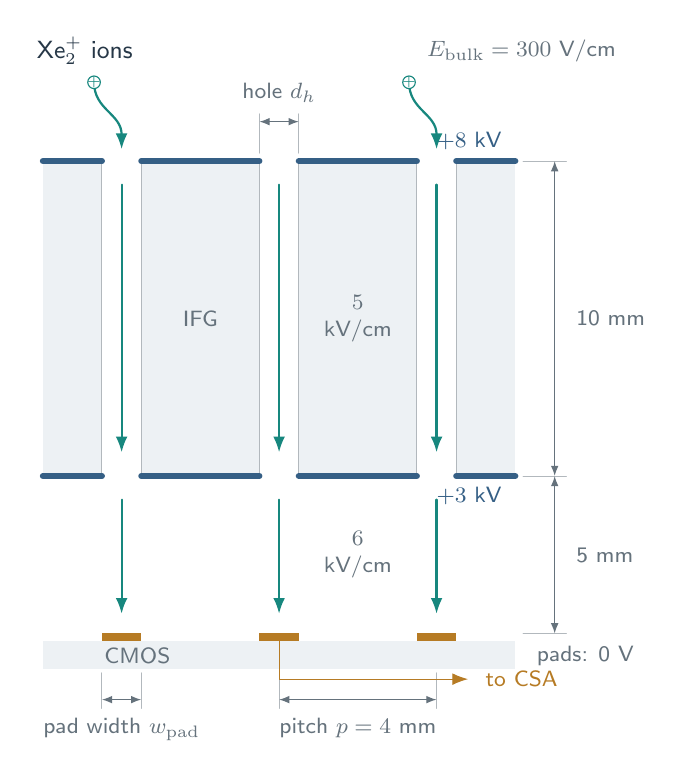
\begin{tikzpicture}[
    font=\sffamily\small, text=ink,
    line cap=round, line join=round,
    wire/.style={draw=ink,line width=.8pt},
    flow/.style={draw=ion,line width=.8pt,-{Latex[length=2mm]}},
    dim/.style={draw=muted,line width=.45pt,{Latex[length=1.3mm]}-{Latex[length=1.3mm]}},
    guide/.style={draw=muted!50,line width=.35pt},
    block/.style={draw=electrode,line width=.8pt,fill=electrode!5,rounded corners=1pt,align=center},
    labeltext/.style={font=\sffamily\footnotesize,text=muted}
]


% Vertical scale: 0.4 drawing cm per physical mm.
% IFG: y=3 to 7 (10 mm); pad surface: y=1 (5 mm gap).
\node[anchor=west] at (.2,8.4) {Xe$_2^+$ ions};
\node[anchor=east,labeltext] at (7.8,8.4) {$E_{\mathrm{bulk}}=300$ V/cm};
\fill[body] (.4,3) rectangle (6.4,7);
\foreach \xc in {1.4,3.4,5.4} {
  \fill[white] ({\xc-.25},3) rectangle ({\xc+.25},7);
  \draw[guide] ({\xc-.25},3)--({\xc-.25},7);
  \draw[guide] ({\xc+.25},3)--({\xc+.25},7);
  \draw[flow] (\xc,6.7)--(\xc,3.3);
  \draw[flow] (\xc,2.7)--(\xc,1.25);
}
\foreach \ya in {3,7} {
  \foreach \xa/\xb in {.4/1.15,1.65/3.15,3.65/5.15,5.65/6.4} {
    \draw[electrode,line width=2.2pt] (\xa,\ya)--(\xb,\ya);
  }
}
\node[anchor=east,text=electrode,font=\sffamily\footnotesize] at (6.35,7.25) {$+8$ kV};
\node[anchor=east,text=electrode,font=\sffamily\footnotesize] at (6.35,2.75) {$+3$ kV};
\node[labeltext] at (2.4,5) {IFG};
\node[labeltext,align=center] at (4.4,5) {$5$\\kV/cm};
\node[labeltext,align=center] at (4.4,2) {$6$\\kV/cm};
\foreach \xc in {1.4,5.4} {
  \draw[flow] ({\xc-.35},8) .. controls ({\xc-.35},7.65) and (\xc,7.6) .. (\xc,7.15);
  \draw[ion,fill=white] ({\xc-.35},8) circle (.08);
  \node[font=\sffamily\tiny,text=ion] at ({\xc-.35},8) {$+$};
}
\draw[guide] (3.15,7.1)--(3.15,7.6);
\draw[guide] (3.65,7.1)--(3.65,7.6);
\draw[dim] (3.15,7.5)--(3.65,7.5);
\node[labeltext,anchor=south] at (3.4,7.62) {hole $d_h$};
\foreach \y in {1,3,7} {\draw[guide] (6.5,\y)--(7.05,\y);}
\draw[dim] (6.9,3)--(6.9,7);
\node[anchor=west,labeltext] at (7.05,5) {10 mm};
\draw[dim] (6.9,1)--(6.9,3);
\node[anchor=west,labeltext] at (7.05,2) {5 mm};
\fill[body] (.4,.55) rectangle (6.4,.9);
\node[labeltext] at (1.6,.72) {CMOS};
\foreach \xc in {1.4,3.4,5.4} {
  \fill[pad] ({\xc-.25},.9) rectangle ({\xc+.25},1);
}
\node[anchor=west,labeltext] at (6.55,.72) {pads: 0 V};
\foreach \x in {3.4,5.4} {\draw[guide] (\x,.5)--(\x,.05);}
\draw[dim] (3.4,.16)--(5.4,.16);
\node[anchor=north,labeltext] at (4.4,.05) {pitch $p=4$ mm};
\foreach \x in {1.15,1.65} {\draw[guide] (\x,.5)--(\x,.05);}
\draw[dim] (1.15,.16)--(1.65,.16);
\node[anchor=north,labeltext] at (1.4,.05) {pad width $w_{\mathrm{pad}}$};
\draw[pad,-{Latex[length=2mm]}] (3.4,.9)--(3.4,.42)--(5.8,.42);
\node[anchor=west,labeltext,text=pad] at (5.9,.42) {to CSA};
\end{tikzpicture}
\end{document}
